\documentclass{article}

% if you need to pass options to natbib, use, e.g.:
     \PassOptionsToPackage{numbers, compress}{natbib}
% before loading neurips_2021

% ready for submission
%\usepackage{neurips_2021}

% to compile a preprint version, e.g., for submission to arXiv, add add the
% [preprint] option:
     \usepackage[preprint]{neurips_2021}

% to compile a camera-ready version, add the [final] option, e.g.:
%     \usepackage[final]{neurips_2021}

% to avoid loading the natbib package, add option nonatbib:
%    \usepackage[nonatbib]{neurips_2021}

%%%%%%%%%%%%%%%%%%%%%%%%%%%%%%%%%%%%%%%%%%%%%%%%%%%%%%%%%%%%
\bibliographystyle{unsrtnat} % <----------- must add for natbib\usepackage{graphicx}
\usepackage{graphicx}
\graphicspath{{images/}}
%%%%%%%%%%%%%%%%%%%%%%%%%%%%%%%%%%%%%%%%%%%%%%%%%%%%%%%%%%%%

\usepackage[utf8]{inputenc} % allow utf-8 input
\usepackage[T1]{fontenc}    % use 8-bit T1 fonts
\usepackage{hyperref}       % hyperlinks
\usepackage{url}            % simple URL typesetting
\usepackage{booktabs}       % professional-quality tables
\usepackage{amsfonts}       % blackboard math symbols
\usepackage{nicefrac}       % compact symbols for 1/2, etc.
\usepackage{microtype}      % microtypography
\usepackage{xcolor}         % colors

\title{DMSN final project: Improve LESSR model structure}

% The \author macro works with any number of authors. There are two commands
% used to separate the names and addresses of multiple authors: \And and \AND.
%
% Using \And between authors leaves it to LaTeX to determine where to break the
% lines. Using \AND forces a line break at that point. So, if LaTeX puts 3 of 4
% authors names on the first line, and the last on the second line, try using
% \AND instead of \And before the third author name.

\author{%
  TENG, LI-CHANG\\
  Department of Electrical Engineering\\
  National Cheng Kung University\\
  \texttt{n26091194@gs.ncku.edu.tw} \\
  % examples of more authors
  \And
  TENG, LI-CHANG\\
  Department of Electrical Engineering\\
  National Cheng Kung University\\
  \texttt{n26091194@gs.ncku.edu.tw} \\
  \AND
  TENG, LI-CHANG\\
  Department of Electrical Engineering\\
  National Cheng Kung University\\
  \texttt{n26091194@gs.ncku.edu.tw} \\
  \And
  TENG, LI-CHANG\\
  Department of Electrical Engineering\\
  National Cheng Kung University\\
  \texttt{n26091194@gs.ncku.edu.tw} \\
%   \And
%   Coauthor \\
%   Affiliation \\
%   Address \\
%   \texttt{email} \\
}

\begin{document}

\maketitle

%%%%%%%%%%%%%%%%%%%%%%%%%%%%%%%%%%%%%%%%%%%%%%%%%%%%%%%%%%%%

\begin{abstract}
    None
    \vspace{2cm}
\end{abstract}

%%%%%%%%%%%%%%%%%%%%%%%%%%%%%%%%%%%%%%%%%%%%%%%%%%%%%%%%%%%%

\section{INTRODUCTION}

Due to the highly practical value,
session-based recommendation attracted researchers’ great attention.
Most of the methods proposed earlier are based on Markov chains or
recurrent neural networks (RNNs). Recently, GNNs have become increasingly
popular and achieved state-of-the-art performance in many tasks.
There are also some attempts to apply GNNs to session-based recommendation.

Although these GNN-based methods obtained exciting results and
offered a new and promising direction for session-based recommendation,
we observe that there are two information loss problems in these methods.
The first information loss problem in the existing GNN-based methods
is called the lossy session encoding problem.
The second information loss problem is called the
ineffective long-range dependency capturing problem where
these GNN-based methods cannot effectively capture all long-range dependencies.

To solve the above problems, author propose a novel GNN model called
LESSR (Lossless Edge-order preserving aggregation
and Shortcut graph attention for Session-based Recommendation).
Through the structure of the original paper,
we found that there are three places with GRU.
We hope to increase the speed of the model by changing the part of GRU.
We change GRU to attention,
then change the model to Transformer,
increase the number of layers and increase pos encoding,
and finally see if the time and accuracy increase.


%%%%%%%%%%%%%%%%%%%%%%%%%%%%%%%%%%%%%%%%%%%%%%%%%%%%%%%%%%%%

\section{RELATED WORK}

A given input session is first converted to a losslessly encoded graph
called edge-order preserving (EOP) multigraph and a shortcut graph
where the EOP multigraph could address the lossy session encoding
problem and the shortcut graph could address
the ineffective long-range dependency capturing problem.
Then, the graphs along with the item embeddings are passed
to multiple edge-order preserving aggregation (EOPA)
and shortcut graph attention (SGAT) layers
to generate latent features of all nodes.
The EOPA layers capture local context information using the EOP multigraph
and the SGAT layers effectively capture long-range dependencies using
the shortcut graph, and the architecture diagram is as figure~\ref{fig:lessr}.

\begin{figure}
    \centering
    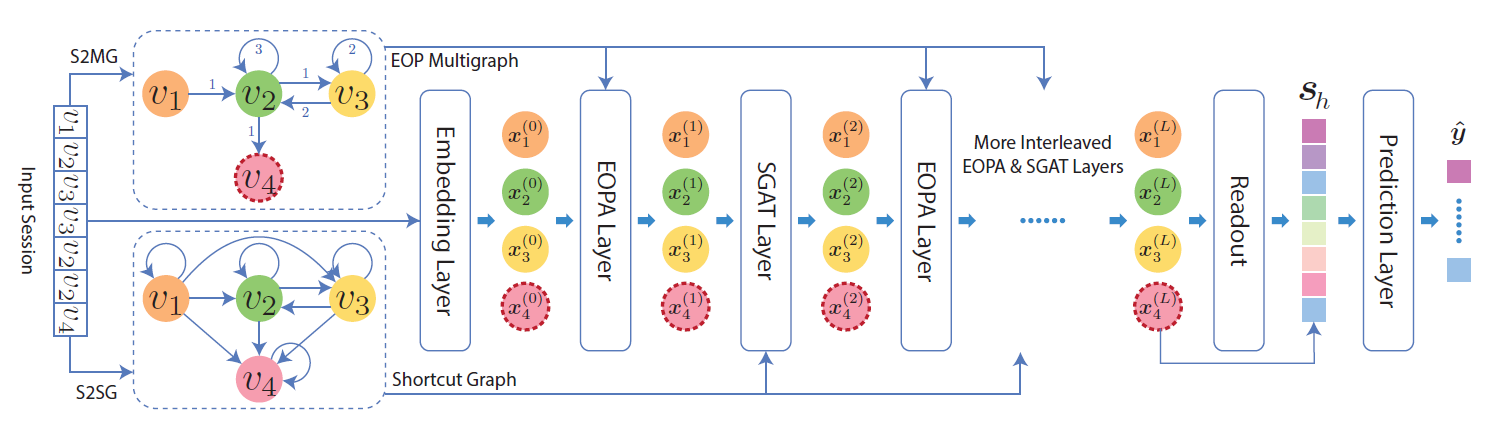
\includegraphics[scale=0.35]{lessr}
    \caption{LESSR structure}
    \label{fig:lessr}
\end{figure}



%%%%%%%%%%%%%%%%%%%%%%%%%%%%%%%%%%%%%%%%%%%%%%%%%%%%%%%%%%%%

\section{PRELIMINARY}

\subsection{GRU}

GRU (Gate Recurrent Unit) is a type of Recurrent Neural Network (RNN).
It is proposed to solve the problems of long-term memory and
gradients in back propagation.
GRU input and output structure:
The input-output structure of GRU is the same as that of ordinary RNN.
There is a current input $x^t$ and the hidden state $h^{t-1}$ passed down
from the previous node. This hidden state contains information
about the previous node.
The GRU structure as shown in figure~\ref{fig:gru}.

\begin{figure}
    \centering
    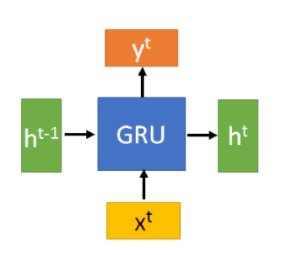
\includegraphics[scale=0.5]{gru}
    \caption{GRU structure}
    \label{fig:gru}
\end{figure}

\subsection{Self-Attention}

For self-attention, the three matrices Q(Query), K(Key), and V(Value) are
all from the same input. First, we have to calculate the dot product
between Q and K, and then in order to prevent the result
from being too large, we will Divide by $\sqrt{d_k}$,
then pass the basis activity function, and finally multiply by V,
it can be expressed by the following formula~\ref{eq:attn}.

\begin{equation}
    \label{eq:attn}
    Attention(Q,K,V)=softmax(\frac{QK^{T}}{\sqrt{d_{k}}})v
\end{equation}

And multi-head means that we can have different Q, K, V representations,
and finally combine the results.

%%%%%%%%%%%%%%%%%%%%%%%%%%%%%%%%%%%%%%%%%%%%%%%%%%%%%%%%%%%%

\section{METHODOLOGY}

\subsection{Transformer Encoder}

In this section, we will introduce the structure of transformer encoder,
which will be used to replace the GRU layer in EOPA
in the following experiments.

\begin{figure}
    \centering
    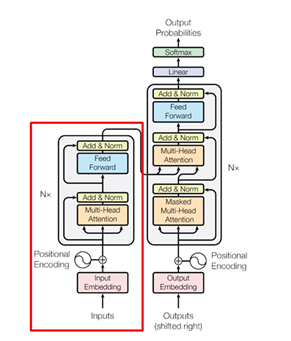
\includegraphics[scale=0.8]{tf}
    \caption{Transformer structure}
    \label{fig:tf}
\end{figure}

Each transformer encoder has two sub-layers.
The first one is Multi-Head Attention layer,
and the second one is a fully connected feed forward layer.
After both layer, we employ residual connection layers and
layer normalization layers. We will specific each layer later.
The Transformer structure is shown in figure~\ref{fig:tf}.

\subsection{Multi-Head Attention}

The first one is the Multi-Head Attention layer.
In this layer our goal is to get attention score from the graphs.
In Multi-Head Attention layer, we have three groups of variables,
Q, k, V, represent query, keys, value respectively.
The number $i$ in these groups (ex: $Q\{q_1, q_2, \dots, q_i\}$)
is decided by how many heads we use. After that,
we will use the following formula to compute the attention weight,
where $d_k$ represents vector dimensionality of k, v and
Z represents final attention weight.
The Multi-Head Attention structure is shown in figure~\ref{fig:multihead}.

\begin{figure}
    \centering
    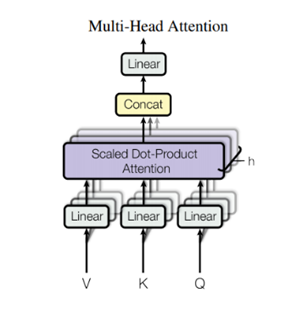
\includegraphics[scale=0.6]{multihead}
    \caption{Multi-Head Attention}
    \label{fig:multihead}
\end{figure}

\subsection{Add \& Norm}

In these layers we use residual connection and layers normalization to
help our model training. With residual connection,
we can let gradient flow directive through the network,
preventing gradient vanishing. As for layers normalization,
it’s effective at stabling the hidden state dynamic our model.
In mathematical definition, residual connection can be simply denoted
by the following formula~\ref{eq:residual}.

\begin{equation}
    \label{eq:residual}
    add(x)=x+sublayer(x)
\end{equation}

On the other hand, layers normalization is much complex.
Assume we give input x over a mini batch size of m,
which is $B={x_1, x_2, \ldots, x_m}$. Each sample x contain K elements.
We first compute the mean and variance of each sample x,
denoted by the following formula~\ref{eq:mu}.

\begin{equation}
    \label{eq:mu}
    \mu_i=
    \frac{1}{K}\Sigma x_{i,k}\sigma_i^2=
    \frac{1}{K}\Sigma{{(x}_{i,k}-\mu_i)}^2
\end{equation}

Then we normalize each sample such that the elements in the sample
have zero mean and unit variance as formula~\ref{eq:norm}.
$\epsilon$ is for numerical stability
in case the denominator becomes zero by chance.

\begin{equation}
    \label{eq:norm}
    x_{i,k}=\frac{{(x}_{i,k}-\mu_i)}{\sqrt{\sigma_i^2-\epsilon}}
\end{equation}

Combining these two layers we simplify its as formula~\ref{eq:layernorm}

\begin{equation}
    \label{eq:layernorm}
    \textrm{LayerNorm}\left(x+\textrm{sublayer}(x)\right)
\end{equation}

Recall that sublayers is Multi-Head Attention and feed forward network.

\subsection{Feedforward Network}

In addition to attend sub-layers,
we employ a fully connected feed-forward network
shown as formula~\ref{eq:ffn} in our encoder.
This consist of two linear transformation with a ReLU activation function.

\begin{equation}
    \label{eq:ffn}
    \textrm{FFN}\left(x\right)=\max{\left(0,xW_1+b_1\right)}W_2+b_2
\end{equation}



%%%%%%%%%%%%%%%%%%%%%%%%%%%%%%%%%%%%%%%%%%%%%%%%%%%%%%%%%%%%

\section{EXPERIMENTS}

In this section, we will introduce experiment setting,
dataset, and analyze the experiment result.
We conducted several experiments to check our hypotheses and evaluate our
model with chosen metric.

\subsection{Dataset}

We choose Diginetica dataset\footnote{\url{https://competitions.codalab.org/competitions/111610}}
following LESSR \cite{chen2020lessr} paper,
which is the CIKM cup 2016 dataset provided by DIGINETICA Crop.
There are 6 files in Diginetica dataset, but we only need the transaction one.
As \cite{chen2020lessr}, we used last week sessions as test data.
We got the same training and test set by following preprocessing method
described in \cite{chen2020lessr}.
Statistics of Diginetica dataset is shown in Table~\ref{data-stats}.

\begin{table}
    \caption{statistics of dataset}
    \label{data-stats}
    \centering
    \begin{tabular}{ll}
        \toprule
        \multicolumn{2}{c}{Diginetica} \\
        \midrule
        No. of Clicks   & 981,620      \\
        No. of Sessions & 777,029      \\
        No. of Items    & 42,596       \\
        Average length  & 4.80         \\
        \bottomrule
    \end{tabular}
\end{table}

\subsection{Baseline and metrics}

We choose \cite{chen2020lessr} as out baseline model,
then we tried to improve model structure in \cite{chen2020lessr} by some changes.
Comparing the metrics to \cite{chen2020lessr},
we could know the change is positive or negative influence.
Following \cite{chen2020lessr},
the metrics we used are HR@20 (Hit Rate) and MRR@20 (Mean Reciprocal Rank).

\subsection{MUTIHEADATTENTION layer}

MUTIHEADATTENTION\footnote{\url{https://pytorch.org/docs/stable/generated/torch.nn.MultiheadAttention.html}}
is a official implemented self-attention layer by pytorch.
Here we replace GRU\footnote{\url{https://pytorch.org/docs/stable/generated/torch.nn.GRU.html}}
layer in EOPA block in \cite{chen2020lessr} by MUTIHEADATTENTION layer.
All settings are the same but GRU now replaced by MUTIHEADATTENTION.
We adjusted num of heads parameter in MUTIHEADATTENTION layer
to see the influence of multi-head attention.

The pytorch official did not implemented positional encoding in
MUTIHEADATTENTION layer, so there is no position information within layer.
To handle this problem we need to do position encoding manually.
We found a official tutorial\footnote{\url{https://pytorch.org/tutorials/beginner/transformer_tutorial.html}}
that manually implemented position encoding,
so we followed the encoding method here.

Table~\ref{Multi-head w/o pos encoding} and Table~\ref{Multi-head with pos encoding}
are the experiment result without and with positional encoding respectively.
It turns out no matter multi-head or positional encoding, can not improve the result.
So in next section we decided to using more complex layer.

\begin{table}
    \caption{Multi-head w/o pos encoding}
    \label{Multi-head w/o pos encoding}
    \centering
    \begin{tabular}{lllll}
        \toprule
        AGG.TYPE & HR@20 & MRR@20 & NDCG@20 & Total impv.  \\
        \midrule
        baseline & 52.82 & 18.3   & 25.93   & -            \\
        Head=1   & 52.65 & 18.25  & 25.85   & -0.903594775 \\
        Head=2   & 52.58 & 18.27  & 25.84   & -0.965396084 \\
        Head=4   & 52.6  & 18.28  & 25.85   & -0.834321462 \\
        Head=8   & 52.63 & 18.28  & 25.87   & -0.700394057 \\
        Head=16  & 52.62 & 18.28  & 25.86   & -0.757891648 \\
        Head=32  & 52.64 & 18.29  & 25.87   & -0.626817026 \\
        \bottomrule
    \end{tabular}
\end{table}

\begin{table}
    \caption{Multi-head with pos encoding}
    \label{Multi-head with pos encoding}
    \centering
    \begin{tabular}{lllll}
        \toprule
        AGG.TYPE & HR@20 & MRR@20 & NDCG@20 & Total impv.  \\
        \midrule
        baseline & 52.82 & 18.3   & 25.93   & -            \\
        Head=1   & 52.57 & 18.26  & 25.83   & -1.077538484 \\
        Head=2   & 52.55 & 18.29  & 25.85   & -0.874337766 \\
        Head=4   & 52.59 & 18.3   & 25.88   & -0.628267962 \\
        Head=8   & 52.62 & 18.29  & 25.87   & -0.664681471 \\
        Head=16  & 52.54 & 18.31  & 25.86   & -0.745415003 \\
        Head=32  & 52.57 & 18.32  & 25.89   & -0.518277422 \\
        \bottomrule
    \end{tabular}
\end{table}

\subsection{TransformerEncoder layer}

In this section, we use transformer encoder
\footnote{\url{https://pytorch.org/docs/stable/generated/torch.nn.TransformerEncoder.html}}
to replace GRU.
TransformerEncoder has a lot of hyperparameter, so we conducted
3 main experiments to tuning the model:
1) dim\_feedforward 2) nhead 3) encoder\_layer.
Also, each main experiments have two sub experiments:
1) w/o pos encoding 2) with pos encoding.

\subsubsection{Dim\_Feedforward Experiment}

In this experiment we fix all hyperprameters but dim\_feedforward.
Table~\ref{dim exp w/o pos encoding} shown the result without
positional encoding.
Table~\ref{dim exp with pos encoding} shown the result with positional encoding.

From Table~\ref{dim exp w/o pos encoding} and Table~\ref{dim exp with pos encoding},
we found that the best dim\_feedforward is setting 512,
whether with pos encoding or not, dimension 512 in both case has a good result,
so we choose dimension 512 for our model in the later experiments.

\begin{table}
    \caption{dim exp w/o pos encoding}
    \label{dim exp w/o pos encoding}
    \centering
    \begin{tabular}{lllll}
        \toprule
        AGG.TYPE   & HR@20 & MRR@20 & NDCG@20 & Total impv.  \\
        \midrule
        baseline   & 52.82 & 18.3   & 25.93   & -            \\
        Dim = 2048 & 52.73 & 18.25  & 25.83   & -0.82926773  \\
        Dim = 1024 & 52.9  & 18.31  & 25.86   & -0.063854988 \\
        Dim = 512  & 52.97 & 18.35  & 26      & 0.827164961  \\
        Dim = 256  & 52.67 & 18.28  & 25.88   & -0.586099799 \\
        Dim = 128  & 52.88 & 18.34  & 25.94   & 0.370737939  \\
        Dim = 64   & 52.84 & 18.39  & 26.01   & 0.83819067   \\
        Dim = 32   & 52.7  & 18.24  & 25.85   & -0.863578471 \\
        Dim = 16   & 52.68 & 18.3   & 25.88   & -0.457877958 \\
        \bottomrule
    \end{tabular}
\end{table}

\begin{table}
    \caption{dim exp with pos encoding}
    \label{dim exp with pos encoding}
    \centering
    \begin{tabular}{lllll}
        \toprule
        AGG.TYPE   & HR@20 & MRR@20 & NDCG@20 & Total impv.  \\
        \midrule
        baseline   & 52.82 & 18.3   & 25.93   & -            \\
        Dim = 2048 & 52.74 & 18.28  & 25.88   & -0.45357424  \\
        Dim = 1024 & 52.86 & 18.3   & 25.88   & -0.117097951 \\
        Dim = 512  & 52.85 & 18.36  & 25.97   & 0.538926994  \\
        Dim = 256  & 52.7  & 18.26  & 25.86   & -0.715723485 \\
        Dim = 128  & 52.89 & 18.37  & 25.95   & 0.592169956  \\
        Dim = 64   & 52.79 & 18.34  & 25.95   & 0.238913304  \\
        Dim = 32   & 52.74 & 18.29  & 25.9    & -0.321798695 \\
        Dim = 16   & 52.6  & 18.36  & 25.92   & -0.127205414 \\
        \bottomrule
    \end{tabular}
\end{table}

\subsubsection{Multi-Head Experiment}

Here we fixed all hyperprameters but nhead to see the influence.
Also, The dim\_feedforward set to 512.
Result without positional encoding shown in
Table~\ref{multi-head exp w/o pos encoding} and result with
positional encoding shown in Table~\ref{multi-head exp with pos encoding}.

Comparing  Table~\ref{multi-head exp w/o pos encoding} and
Table~\ref{multi-head exp with pos encoding},
We found the metrics without positional encoding are usually
better than the other one.
So positional information might not a critical info in this scenario.

Note that best performance appeared when nhead set to 8 with positional encoding.

\begin{table}
    \caption{multi-head exp w/o pos encoding}
    \label{multi-head exp w/o pos encoding}
    \centering
    \begin{tabular}{lllll}
        \toprule
        AGG.TYPE & HR@20 & MRR@20 & NDCG@20 & Total impv. \\
        \midrule
        baseline & 52.82 & 18.3   & 25.93   & -           \\
        nhead=1  & 52.97 & 18.35  & 26      & 0.827164961 \\
        nhead=2  & 52.77 & 18.37  & 25.95   & 0.364983285 \\
        nhead=4  & 52.98 & 18.35  & 26      & 0.846097184 \\
        nhead=8  & 52.87 & 18.37  & 25.96   & 0.592870879 \\
        nhead=16 & 52.78 & 18.37  & 25.97   & 0.461046244 \\
        nhead=32 & 52.92 & 18.41  & 25.97   & 0.944676596 \\
        \bottomrule
    \end{tabular}
\end{table}

\begin{table}
    \caption{multi-head exp with pos encoding}
    \label{multi-head exp with pos encoding}
    \centering
    \begin{tabular}{lllll}
        \toprule
        AGG.TYPE & HR@20 & MRR@20 & NDCG@20 & Total impv. \\
        \midrule
        baseline & 52.82 & 18.3   & 25.93   & -           \\
        nhead=1  & 52.85 & 18.36  & 25.97   & 0.538926994 \\
        nhead=2  & 52.7  & 18.31  & 25.91   & -0.2496726  \\
        nhead=4  & 52.88 & 18.38  & 25.98   & 0.743578647 \\
        nhead=8  & 52.87 & 18.41  & 26.03   & 1.081407692 \\
        nhead=16 & 52.82 & 18.35  & 25.96   & 0.388920149 \\
        nhead=32 & 52.75 & 18.35  & 25.95   & 0.217829222 \\
        \bottomrule
    \end{tabular}
\end{table}

\subsubsection{Num-Layers Experiment}

Here all hyperprameters was fixed but num\_layers will be change.
The dim\_feedforward was set to 512 and nhead was set to 1.
Table~\ref{num-layers exp w/o pos} and Table~\ref{num-layers exp with pos}
shown the result without and with positional encoding respectively.

We found that whether transformer encoder with positional encoding or not,
it has similar trend that performance decreased as layers increased.
And we found as layers increased, model's inference time also increased.

\begin{table}
    \caption{num-layers exp w/o pos}
    \label{num-layers exp w/o pos}
    \centering
    \begin{tabular}{lllll}
        \toprule
        AGG.TYPE & HR@20 & MRR@20 & NDCG@20 & Total impv.  \\
        \midrule
        baseline & 52.82 & 18.3   & 25.93   & -            \\
        layer=1  & 52.97 & 18.35  & 26      & 0.827164961  \\
        layer=2  & 52.72 & 18.41  & 25.93   & 0.41177067   \\
        layer=3  & 52.69 & 18.4   & 25.95   & 0.37745993   \\
        layer=4  & 52.69 & 18.33  & 25.89   & -0.236445941 \\
        layer=6  & 52.65 & 18.13  & 25.72   & -2.060682268 \\
        layer=8  & 52.24 & 17.96  & 25.48   & -4.691433984 \\
        layer=16 & 52.11 & 17.77  & 25.34   & -6.515719401 \\
        \bottomrule
    \end{tabular}
\end{table}

\begin{table}
    \caption{num-layers exp with pos}
    \label{num-layers exp with pos}
    \centering
    \begin{tabular}{lllll}
        \toprule
        AGG.TYPE & HR@20 & MRR@20 & NDCG@20 & Total impv.  \\
        \midrule
        baseline & 52.82 & 18.3   & 25.93   & -            \\
        layer=1  & 52.85 & 18.36  & 25.97   & 0.538926994  \\
        layer=2  & 52.77 & 18.41  & 25.96   & 0.622127888  \\
        layer=3  & 52.72 & 18.34  & 25.88   & -0.163569833 \\
        layer=4  & 52.84 & 18.32  & 25.9    & 0.031457958  \\
        layer=6  & 52.8  & 18.18  & 25.78   & -1.272082675 \\
        layer=8  & 52.3  & 17.95  & 25.46   & -4.709616194 \\
        layer=16 & 52.04 & 17.81  & 25.37   & -6.313969619 \\
        \bottomrule
    \end{tabular}
\end{table}

%%%%%%%%%%%%%%%%%%%%%%%%%%%%%%%%%%%%%%%%%%%%%%%%%%%%%%%%%%%%

\section{CONCLUSION}

In our experiments, no matter with positional encoding or not,
the performance of MUTIHEADATTENTION is worse than GRU,
although using MUTIHEADATTENTION is slightly fast.
In multi-head experiment of TransformerEncoder,
we found there is no distinct trend about num of head,
also we found when TransformerEncoder stacking more layers,
model's performance will decreased, this means the model is over-fitting,
moreover, evaluate time will increased, this cause training time getting longer.

After several experiments, we found that TransformerEncoder can improve
model performance by replacing GRU in EOPA layer,
but the parameter of TransformerEncoder need in proper setting.
In SGAT and Readout layer, we tried to change the attention mechanisms,
but we didn't got a good result.
This might because attention mechanisms is dependent on model structure and data,
it won't be useful if we just replace attention mechanisms from different paper.

Finally the best result we got is when layer=1 and nhead=8
with positional encoding, total improvement of three metrics is  1.08\%,
although there is still a space for improvements in this model.
The result is a acceptable to us because we didn't change the model structure
so much but just change a layer inside EOPA block.
If we could modify SGAT and Readout layer's attention mechanisms
to multi-head attention, we might get a better result.


%%%%%%%%%%%%%%%%%%%%%%%%%%%%%%%%%%%%%%%%%%%%%%%%%%%%%%%%%%%%


\bibliography{refer}


\end{document}